\documentclass[10pt]{article}
\usepackage{amsmath,amsfonts,times}
\usepackage{graphicx,color,tikz,pgfplots}
\usepackage[paperwidth=6cm,paperheight=8cm,lmargin=0in,rmargin=0in,tmargin=0.in,bmargin=0.in]{geometry}
\usepackage{bm}
\usetikzlibrary{arrows,shadings,shapes.arrows,decorations.pathreplacing,calc, positioning}
\usepgfplotslibrary{fillbetween}

\pgfplotsset{
  compat=newest
}

\newlength{\dx}
\setlength{\dx}{1.5cm}

\newlength{\circleRadius}
\setlength{\circleRadius}{0.95\dx}

\definecolor{outside}{rgb}{0, 1, 0}
\definecolor{cutcell}{rgb}{0, 0.5, 1}
\definecolor{inside}{rgb}{1, 0, 0}

\tikzset{
  edge/.style={draw=black},
  tree/.style={thick, draw=black, solid, ->},
  bvh/.style={draw=black, minimum width=5mm, minimum height=5mm, rectangle, rounded corners, very thick},
  vertex/.style={circle, inner sep=0pt, minimum width=4pt, draw=black, fill=white, node contents={}},
  point/.style={circle, inner sep=0pt, minimum width=6pt, thick, draw=black, fill=white},
  root/.style={ultra thick, densely dashed, draw=black},
  R1/.style={very thick, draw=black, fill=green!50!white, solid, fill opacity=0.4},
  R2/.style={very thick, draw=black, fill=blue!50!white, solid, fill opacity=0.4},
}

\begin{document}
\centering
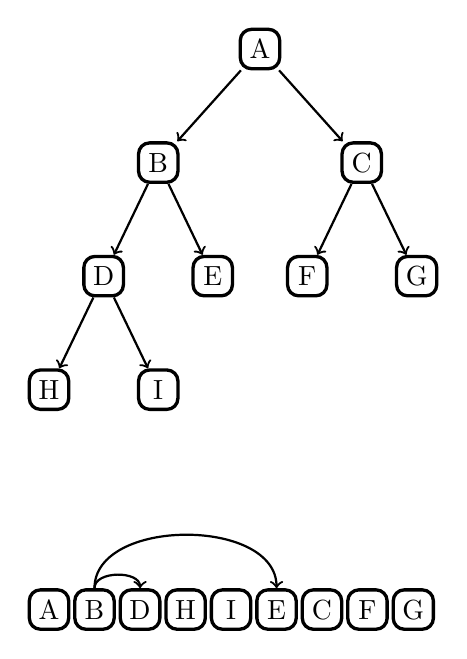
\begin{tikzpicture}

    %% \draw[root] (-2.55\dx,-1.166\dx) rectangle (1.3\dx, 1.8\dx);
    %% \draw[left] (-2.25\dx,-0.766\dx) rectangle (-0.5\dx, 1.5\dx);
    %% \draw[right] (-0.7\dx,-0.866\dx) rectangle (1\dx, 1.1\dx);
    %% \draw[R1] (-0.7\dx,0\dx) rectangle (1\dx, 1.1\dx);
    %% \draw[R2] (-0.7\dx,-0.866\dx) rectangle (1\dx, 0.134\dx);        

    %% \node (v0) at (0.1\dx,0.2\dx) [vertex];
    %% \node (v1) at (\dx, 0) [vertex];
    %% \node (v2) at (0.5\dx, 0.866\dx) [vertex];
    %% \node (v3) at (-0.5\dx, 1.1\dx) [vertex];
    %% \node (v4) at (-0.7\dx, 0) [vertex];
    %% \node (v5) at (-0.5\dx, -0.766\dx) [vertex];
    %% \node (v6) at (0.5\dx, -0.866\dx) [vertex];

    %% \node (v7) at (-1.5\dx, 0.866\dx) [vertex];
    %% \node (v8) at (-1.25\dx, 1.5\dx) [vertex];
    %% \node (v9) at (-2.25\dx, -0.5\dx) [vertex];

    %% \draw[edge] (v0)--(v1);
    %% \draw[edge] (v0)--(v2);
    %% \draw[edge] (v0)--(v3);
    %% \draw[edge] (v0)--(v4);
    %% \draw[edge] (v0)--(v5);
    %% \draw[edge] (v0)--(v6);

    %% \draw[edge] (v1)--(v2)--(v3)--(v4)--(v5)--(v6)--(v1);

    %% \draw[edge] (v3)--(v8)--(v7)--(v3);
    %% \draw[edge] (v4)--(v7)--(v3)--(v4);
    %% \draw[edge] (v9)--(v4);
    %% \draw[edge] (v9)--(v5);
    %% \draw[edge] (v9)--(v7);

  \node[bvh, alias=A                ] at (3.5\dx, 1.4\dx) {A};
  \node[bvh, alias=B, below left =0.6\dx and 0.5\dx of A] {B};  
  \node[bvh, alias=C, below right=0.6\dx and 0.5\dx of A] {C};
  \node[bvh, alias=D, below left =0.6\dx and 0.1\dx of B] {D};
  \node[bvh, alias=E, below right=0.6\dx and 0.1\dx of B] {E};
  \node[bvh, alias=F, below left =0.6\dx and 0.1\dx of C] {F};
  \node[bvh, alias=G, below right=0.6\dx and 0.1\dx of C] {G};
  \node[bvh, alias=H, below left =0.6\dx and 0.1\dx of D] {H};
  \node[bvh, alias=I, below right=0.6\dx and 0.1\dx of D] {I};          

  \path[tree] (A) to (B);
  \path[tree] (A) to (C);

  \path[tree] (B) to (D);
  \path[tree] (B) to (E);

  \path[tree] (C) to (F);
  \path[tree] (C) to (G);

  \path[tree] (D) to (H);
  \path[tree] (D) to (I);  

  \node[bvh, alias=AA, anchor=north, below=1.5\dx of H] {A};
  \node[bvh, alias=BB, anchor=west, right=1pt of AA] {B};
  \node[bvh, alias=DD, anchor=west, right=1pt of BB] {D};
  \node[bvh, alias=HH, anchor=west, right=1pt of DD] {H};
  \node[bvh, alias=II, anchor=west, right=1pt of HH] {I};
  \node[bvh, alias=EE, anchor=west, right=1pt of II] {E};
  \node[bvh, alias=CC, anchor=west, right=1pt of EE] {C};
  \node[bvh, alias=FF, anchor=west, right=1pt of CC] {F};
  \node[bvh, alias=GG, anchor=west, right=1pt of FF] {G};

  \draw[thick, black,->] (BB.north) to [out=90, in=90] (DD.north);
  \draw[thick, black,->] (BB.north) to [out=90, in=90] (EE.north);  
\end{tikzpicture}

\end{document} 
